%%
%% This is file `sample-manuscript.tex',
%% generated with the docstrip utility.
%%
%% The original source files were:
%%
%% samples.dtx  (with options: `manuscript')
%% 
%% IMPORTANT NOTICE:
%% 
%% For the copyright see the source file.
%% 
%% Any modified versions of this file must be renamed
%% with new filenames distinct from sample-manuscript.tex.
%% 
%% For distribution of the original source see the terms
%% for copying and modification in the file samples.dtx.
%% 
%% This generated file may be distributed as long as the
%% original source files, as listed above, are part of the
%% same distribution. (The sources need not necessarily be
%% in the same archive or directory.)
%%
%% The first command in your LaTeX source must be the \documentclass command.
\documentclass[acmsmall,review,nonacm]{acmart}\settopmatter{printfolios=true,printccs=false,printacmref=false}

%%
%% \BibTeX command to typeset BibTeX logo in the docs
\AtBeginDocument{%
  \providecommand\BibTeX{{%
    \normalfont B\kern-0.5em{\scshape i\kern-0.25em b}\kern-0.8em\TeX}}}

%% Rights management information.  This information is sent to you
%% when you complete the rights form.  These commands have SAMPLE
%% values in them; it is your responsibility as an author to replace
%% the commands and values with those provided to you when you
%% complete the rights form.
\setcopyright{acmcopyright}
\copyrightyear{2018}
\acmYear{2018}
\acmDOI{10.1145/1122445.1122456}

% for code
\usepackage{listings}
\usepackage{lipsum}
\usepackage{xcolor}
\usepackage{minted}
\RecustomVerbatimEnvironment{Verbatim}{BVerbatim}{}

% tables
\usepackage{multirow}


%% These commands are for a PROCEEDINGS abstract or paper.
\acmConference[Woodstock '18]{Woodstock '18: ACM Symposium on Neural
  Gaze Detection}{June 03--05, 2018}{Woodstock, NY}
\acmBooktitle{Woodstock '18: ACM Symposium on Neural Gaze Detection,
  June 03--05, 2018, Woodstock, NY}
\acmPrice{15.00}
\acmISBN{978-1-4503-XXXX-X/18/06}


%%
%% Submission ID.
%% Use this when submitting an article to a sponsored event. You'll
%% receive a unique submission ID from the organizers
%% of the event, and this ID should be used as the parameter to this command.
%%\acmSubmissionID{123-A56-BU3}

%%
%% The majority of ACM publications use numbered citations and
%% references.  The command \citestyle{authoryear} switches to the
%% "author year" style.
%%
%% If you are preparing content for an event
%% sponsored by ACM SIGGRAPH, you must use the "author year" style of
%% citations and references.
%% Uncommenting
%% the next command will enable that style.
%%\citestyle{acmauthoryear}

%%
%% end of the preamble, start of the body of the document source.
\begin{document}

%%
%% The "title" command has an optional parameter,
%% allowing the author to define a "short title" to be used in page headers.
\title{Distilling Sparse Linear Algebra}

%%
%% The "author" command and its associated commands are used to define
%% the authors and their affiliations.
%% Of note is the shared affiliation of the first two authors, and the
%% "authornote" and "authornotemark" commands
%% used to denote shared contribution to the research.
\author{Aleksey Tyurin}
% \authornote{Both authors contributed equally to this research.}
\email{aleksey.tyurinspb@gmail.com}
% \orcid{1234-5678-9012}
% \author{G.K.M. Tobin}
% \authornotemark[1]
% \email{webmaster@marysville-ohio.com}
\affiliation{%
  \institution{Saint Petersburg State University}
%   \streetaddress{P.O. Box 1212}
  \city{Saint Petersburg}
%   \state{Ohio}
  \country{Russia}
%   \postcode{43017-6221}
}

\newcommand\todo[1]{{\color{violet}#1}}
\newcommand\db[1]{{\color{red}#1}}
\newcommand\question[1]{{\color{cyan}#1}}

%%
%% By default, the full list of authors will be used in the page
%% headers. Often, this list is too long, and will overlap
%% other information printed in the page headers. This command allows
%% the author to define a more concise list
%% of authors' names for this purpose.
% \renewcommand{\shortauthors}{Trovato and Tobin, et al.}

%%
%% The abstract is a short summary of the work to be presented in the
%% article.


% \begin{abstract}

% Sparse linear algebra is a great framework to tackle a wide variety of problem but in practice its implementations suffer from being memory-bound. Thus a number of optimizations has been proposed towards the reduction of the number of memory accesses. This work proposes an approach to employ distillation to provide such optimizations. It provides some benchmarks and describes the directions of future work. 
  
% \end{abstract}

%%
%% The code below is generated by the tool at http://dl.acm.org/ccs.cfm.
%% Please copy and paste the code instead of the example below.
%%
\begin{CCSXML}
<ccs2012>
 <concept>
  <concept_id>10010520.10010553.10010562</concept_id>
  <concept_desc>Computer systems organization~Embedded systems</concept_desc>
  <concept_significance>500</concept_significance>
 </concept>
 <concept>
  <concept_id>10010520.10010575.10010755</concept_id>
  <concept_desc>Computer systems organization~Redundancy</concept_desc>
  <concept_significance>300</concept_significance>
 </concept>
 <concept>
  <concept_id>10010520.10010553.10010554</concept_id>
  <concept_desc>Computer systems organization~Robotics</concept_desc>
  <concept_significance>100</concept_significance>
 </concept>
 <concept>
  <concept_id>10003033.10003083.10003095</concept_id>
  <concept_desc>Networks~Network reliability</concept_desc>
  <concept_significance>100</concept_significance>
 </concept>
</ccs2012>
\end{CCSXML}

\ccsdesc[500]{Computer systems organization~Embedded systems}
\ccsdesc[300]{Computer systems organization~Redundancy}
\ccsdesc{Computer systems organization~Robotics}
\ccsdesc[100]{Networks~Network reliability}

%%
%% Keywords. The author(s) should pick words that accurately describe
%% the work being presented. Separate the keywords with commas.
% \keywords{datasets, neural networks, gaze detection, text tagging}


%%
%% This command processes the author and affiliation and title
%% information and builds the first part of the formatted document.
\maketitle

\section{Introduction}
Linear algebra is a great instrument for solving a wide variety of problems utilizing matrices and vectors for data representation and analysis with the help of highly optimized routines. But in reality matrices in many applications are often sparse, incurring both computational and storage inefficiencies, requiring an unnecessarily large storage, occupied by zero elements, and a large number of operations on zeroes, where the result is obviously known beforehand. 
The traditional approach to address these inefficiencies is to compress the
matrix and store only the non-zero elements, and then operate only
on the non-zero values.
It makes the techniques of matrix compressed representation and sparse linear algebra to be the effective way of tackling problems in areas including but not limited to graph analysis~\cite{GAILLA}, computational biology~\cite{compBio} and machine learning~\cite{Kepner_2017}.

% And whilst the matrices involved in a vast diversity of modern applications, e.g., recommender~\cite{gupta2020architectural,amazon} systems and graph analysis~\cite{graph1,graph2}, consist of a large number of elements, the major part of them are zeros.

% Such a high sparsity incurs 
% Thus, the effect of matrices tending to be sparse in many applications makes the techniques of matrix compressed representation and sparse linear algebra to be the effective way of tackling problems in areas including but not limited to graph analysis~\cite{GAILLA}, computational biology~\cite{compBio} and machine learning~\cite{Kepner_2017}.

\emph{GraphBLAS}~\cite{buluc2017graphblas} standard defines sparse linear algebra building blocks useful to express algorithms for already mentioned areas in a uniform way in terms of sparse matrix and vector operations over some semiring. These include matrix/vector multiplication, element-wise operations (e-wise for short), kronecker product, masking, i.e. taking a subset of elements that satisfies the mask or its complement, and are sufficient to express a lot of algorithms, e.g. \emph{PageRank}, \emph{Breadth-First-Search}, \emph{Sparse Deep Neural Network}~\cite{SparseDNN}.

% Sparse linear algebra defines building blocks for expressing algorithms for already mentioned areas in a uniform way in terms of sparse matrix and vector operations over some semiring. 
% Once such blocks are implemented in software (or hardware) a myriad of expressible algorithms could be tuned and optimized at once by optimizing and tuning the building blocks.
% \emph{GraphBLAS}~\cite{buluc2017graphblas} standard summarizes such blocks, including but not limited to matrix/vector multiplication, element-wise operations (e-wise for short), kronecker product, masking, i.e. taking a subset of elements that satisfies the mask or its complement. These are sufficient to express a lot of algorithms, e.g. \emph{PageRank}, \emph{Breadth-First-Search}, \emph{Sparse Deep Neural Network}~\cite{SparseDNN}. The parameterizability by a semiring is the key to expressivity since the behaviour of each operation is fully customized.
% \emph{GraphBLAS}~\cite{buluc2017graphblas} standard,
% There are several implementations of GraphBLAS standard showing decent performance for both GPU~\cite{yang2020graphblast} and CPU~\cite{SuiteSparse} backends with one of them already speeding up graph database queries~\cite{redis}.
% The standard itself is a C API specification that standardizes sparse linear algebra building blocks initially for graph computations, but nevertheless applicable in other areas. 
% It translates mathematical specification to API that could be efficiently implemented in hardware or software. 
% Also it is the only such specification and has been completed by researchers from the field of high-performance graph algorithms based on sparse linear algebra. 
% The specification further gives the means for interoperation with vertex-centric libraries, which potentially makes it a crucial component in the future ecosystem of big graphs~\cite{sakr2020future}.
% A list of operations provided by the standard constitutes (the list is not exhaustive) matrix/vector multiplication, element-wise operations (e-wise for short), kronecker product, masking, i.e. taking a subset of elements that satisfies the mask or its complement. These are sufficient to express a lot of algorithms, e.g. \emph{PageRank}, \emph{Breadth-First-Search}, \emph{Sparse Deep Neural Network}~\cite{SparseDNN}. Notably each operation is parameterizable by a semiring, which is the key to expressivity since the behaviour of each operation is fully customized.

However sparse computations appear to have a low arithmetic-to-memory operations intensity, meaning that the main bottleneck of sparse-algorithms is the sparse representation itself that induces pointer-chasing. Thus, a number of optimizations have been identified~\cite{yang2020graphblast}, whose aim is to reduce the intensity of memory accesses and the one considered in this work is \emph{fusion}. \emph{Fusion} simply stands for removal of intermediate data structures, namely those that are first constructed and then deconstructed. There are two types of fusion that we are interested in.

\emph{Mask fusion}. Ahead-of-time masking could reduce the number of memory accesses in case of, e.g., matrix-vector multiplication by taking only the elements of interest.
% and prevent memory blow-up in case of matrix-matrix multiplication: the multiplication of two sparse matrices could produce an order of magnitude
% more non-zeroes in the output matrix compared with the two input matrices, hence the mask could limit the output number of non-zeroes, thus preventing out-of-memory errors.
In order to achieve such a behavior, a mask should be fused (i.e. transformed into a single operation) with the corresponding operation, for the operation to perform computations only for the elements in the mask. The effect of masking in case of sparse matrix-dense vector multiplication could be seen in figure~\ref{fig:fusion}. Ahead-of-time masking reduces the number of memory accesses from 8 to 3.
% Vectors are usually stored both in sparse and dense formats, hence masking could always be performed making sparse matrix-dense vector multiplication faster than sparse matrix-sparse vector multiplication in virtue of implementation details.

\begin{figure}
    \centering
    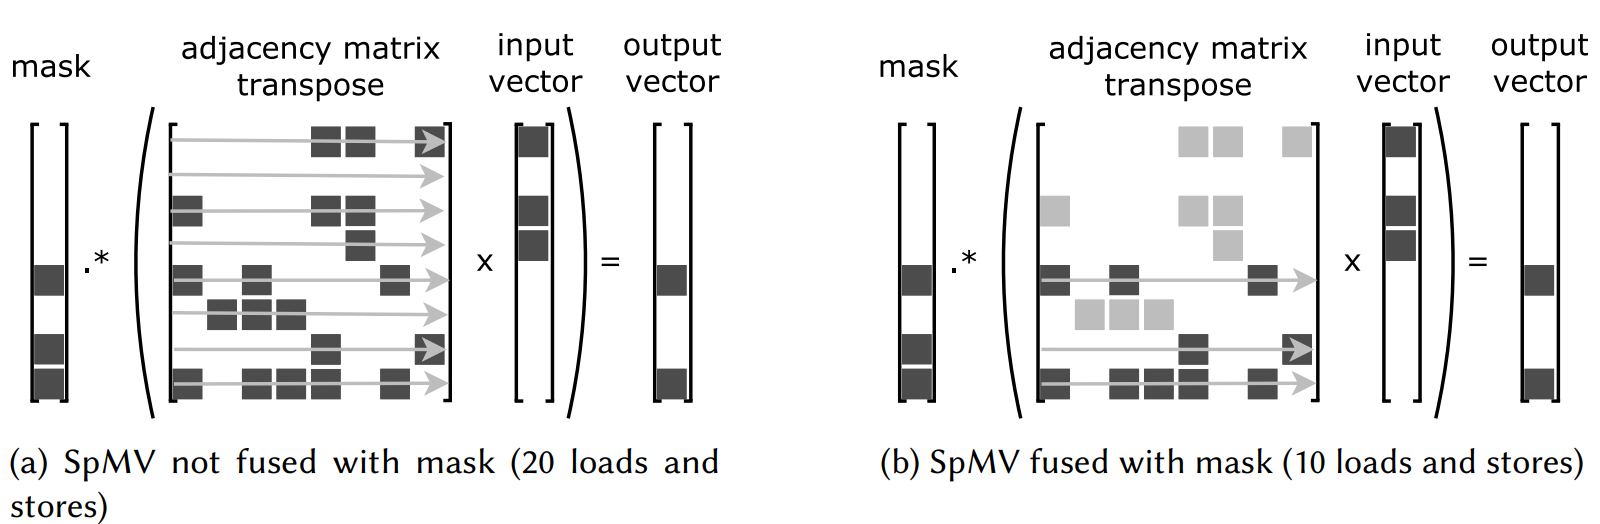
\includegraphics[width=0.75\linewidth]{figures/MaskFusion.png}
    \caption{Mask fusion example~\cite{yang2020graphblast}}
    \label{fig:fusion}
\end{figure}

\emph{Kernel fusion}. 
% Mask fusion is a special case of kernel fusion. 
Kernel fusion is responsible for fusing arbitrary operations. In the case of loop-based programming fusion simply stands for joining several loops into one to increase memory locality and reduce the number of required iterations. It is a crucial technique in dense applications and is usually followed by a stage of \emph{polyhedral analysis}. This is extensively exploited in frameworks like TensorFlow and its XLA compiler~\cite{TensorFlowXLA}. A motivating example for general fusion could be seen in listing~\ref{listing:fusion}\footnote{The original excerpt is in C++, it is rewritten to ease the demonstration. Call-by-value is assumed.}, which is a snippet (simplified for demonstration) from Luby’s maximal independent set algorithm implementation~\cite{SuiteSparseOnly}. As could be seen it is a series of  e-wise matrix additions: two consecutive element-wise operations could be fused into one, so \texttt{new\_members} matrix creation and further iterations are reduced. 

Some general-purpose solutions exists that support fusion, e.g., \cite{Futhark} which are based on map/reduce semantics. But in order to support sparse operations they should be able to fuse across index arithmetic, which is not the case. Also at the moment neither ~\cite{SuiteSparse}  nor ~\cite{yang2020graphblast} have adopted the fusion in their implementations. In this work we propose an approach to support fusion for such applications and outline the overall solution design.

% \begin{listing}
% \centering
% \caption{Excerpt from Luby’s maximal independent set algorithm implementation}
% \label{listing:fusion}
% \begin{minted}[fontsize=\small]{C++}

% // select node if its probability is > than all its active neighbors
% GrB_eWiseAdd (new_members, NULL, GrB_GT_FP64, prob, neighbor_max) ;
% // add new members to independent set.
% GrB_eWiseAdd (iset, NULL, GrB_LOR, iset, new_members) ;

% \end{minted}
% \end{listing}



\begin{listing}
\centering
\caption{Excerpt from Luby’s maximal independent set algorithm implementation}
\label{listing:fusion}
\begin{minted}[fontsize=\footnotesize]{Haskell}

...
-- select node if its probability is > than all its active neighbors

-- @gt is '>' operation, @lor is logical or 
let new_members = eWiseAdd gt prob neighbor_max
    iset' = eWiseAdd lor iset new_members in 
    
...

\end{minted}
\end{listing}

% \begin{table}[t]
%     \centering
%     \begin{tabular}{ |c|c|c|c| } 
% \hline
% Function & Description & Notation \\
% \hline
% \texttt{GrB\_mxm} & matrix-matrix mult. & $C \langle M \rangle = AB$ \\ 
% \texttt{GrB\_eWiseMult} & element-wise, set union &
% $C\langle M \rangle = A \otimes B$\\ 
% \texttt{GrB\_eWiseAdd} & element-wise, set-intersection  & $C \langle M \rangle = A \oplus B$ \\
% \texttt{GrB\_apply} & apply unary op. & $C\langle M \rangle = f(A)$\\
% \hline
% \end{tabular}
%     \caption{Some of the GraphBLAS operations}
%     \label{tab:table_blass}
% \end{table}

\section{Solution}

The problem of intermediate data structures is natural for functional programming and
% where its definition is slightly more formal.
% An intermediate data structure is a structure which is created using a constructor
% application, and is subsequently decomposed as the selector in a
% \texttt{case} expression.
a number of approaches for fusion has been designed, namely \emph{partial evaluation, deforestation, supercompilation, distillation} \cite{jones, WADLER1990231, supercompilation, distillation}. In this work we will focus on \emph{distillation} since it is able to produce a superlinear improvement for the program being optimized~\cite{distillation}.

For succesful fusion the compressed representation should be fuseable, so it should avoid indexing and be natural to functional paradigm. A quad-tree representation~\cite{qtree} looks promising in this case. The implementation of this compressed representation as an algebraic data type could be seen in listing~\ref{lst:fusionhosc}, it recursively splits a matrix into four submatrices. Turning back to the successive e-wise matrix additions example, distillation successfully fuses them into one operation where each matrix is iterated only once as also could be seen in listing~\ref{lst:fusionhosc}. 

If we now define the notion of \textbf{intermediate data structure} as the number of times a constructor term within \texttt{case} context is encountered during the reduction of the top-level term, i.e. the number of times something is deconstructed with pattern-matching, we could see that the fusion also produces a more effective program, as it could be seen in the table~\ref{tab:table_distill}, where $x / y$ are reductions, the number of steps to reduce the term to its normal form, and the number of intermediate structures respectively, the numbers at top are the orders of input matrices. Each example firstly was evaluated using the interpreter that counts the number of reductions and intermediate structures. Then it was distilled\footnote{The distiller from~\cite{distillation} was used} and evaluated again. Matrices/masks have been taken from~\cite{Florida}, converted to q-tree representation and embedded instead of free variables into the corresponding functions. The full list of benchmarks could be found here~\cite{YaccPOT}.

It could be noted that \texttt{case }$c\: e_0 \ldots e_n$, where $c$ is a constructor, essentially performs a memory read, so the optimization reduces the number of eventual memory reads and corresponding writes as well. Another practical example is masking of a kronecker product, since kronecker product performs more operations than matrix-vector multiplication, here it is a more representative example that shows the benefits of masking-fusion. The benefit of optimization is up to \textbf{2x} in terms of reductions and up to \textbf{1.3x} in terms of intermediate structures, hence it could be stated that distillation is applicable to optimize sparse computations and could be able to speed up practical algorithms like Luby's maximal set. The future work and overall idea behind this is described in the next section. 


% \url{https://github.com/YaccConstructor/Distiller}.



\begin{listing}

\begin{minted}[fontsize=\footnotesize]{Haskell}
-- @QNone stands for submatrix which elements are zeroes
data QTree a = QNone  
               | QVal a 
               | QNode (QTree a) (QTree a) (QTree a) (QTree a) 
main = ...
        let new_members = eWiseAdd gt prob neighbor_max 
            iset' = eWiseAdd lor iset new_members in
       ...
--gets fused into
main = ...

    let iset' = case iset of
                ... -> case neighbor_max of
                    ... -> case prob of ...
-- @new_members has been eliminated
\end{minted}
\caption{Fusion by means of distillation}
\label{lst:fusionhosc}

\end{listing}


% \begin{table}[t]
%     \centering
%     \begin{tabular}{ |c|c|c|c|c|c| } 
% \hline
% Function & Description & Reductions & Allocations & \# of non-zeroes \\
% \hline
% \multirow{2}{10em}{E-wise successive additions} & Original & 107 & 22 & 2\\ 
% & Distilled & 44 & 14 & 2\\
% \hline
% \multirow{2}{10em}{Kronecker with masking} & Original & 213 & 45 & 2\\ 
% & Distilled & 108 & 25 & 2\\
% \hline
% \end{tabular}
%     \caption{Distillation results}
%     \label{tab:table_distill}
% \end{table}

\begin{table}[t]
    \centering
    \begin{tabular}{ |c|c|c|c|c|c| } 
\hline
\multirow{2}{10em}{Function} & \multirow{2}{5em}{Description} & \multicolumn{3}{c}{\# of non-zeroes}\vline\\
\cline{3-5}
{}&{} & $10^1$ & $10^2$ & $10^3$ \\
\hline
\multirow{2}{10em}{E-wise successive additions} & Original & 107 / 22 & 11293 / 1852 & 139851 / 20351\\ 
& Distilled & 44 / 14 & 6129 / 1433 & 89215 / 15061\\
\hline
\multirow{2}{10em}{Kronecker with masking} & Original & 213 / 45 & 535125 / 92470 & 6968317 / 1220816\\ 
& Distilled & 108 / 25 & 367868 / 67110 & 3974610 / 867137\\
\hline
\end{tabular}
    \caption{Distillation results}
    \label{tab:table_distill}
\end{table}




\section{Future work}

The obvious disadvantage of this approach is that it requires a special domain-specific language amenable to distillation, so it could hardly be integrated into existing implementations like~\cite{SuiteSparse, yang2020graphblast}. However, typical CPUs and GPUs are proven to be underutilized~\cite{Florida,leskovec2016snap,Song_2016,zhang2020sparch}, i.e., their computing units do not achieve peak performance, suffering from the irregularity of memory accesses incurred by sparsity, so a possible direction could be to design a domain-specific co-processor that is able to execute this distillation-amenable language. Such an approach has found a successful application in image processing~\cite{halide,redgrave2018pixel}, programmable networks~\cite{barefoot} and machine learning~\cite{GoogleTPU,TensorFlowXLA}.

Notably, in~\cite{Edwards2019FHWP} a framework is proposed that is capable of transforming arbitrary Haskell programs into hardware description. It provides datatype-specific memory spaces and divide-and-conquer optimizations (since q-tree representation is divide-and-conquer by its natures, it is a good fit). Each \texttt{case }$c\: e_0 \ldots e_n$ expression is generated as an explicit memory read of $c$ and hence distillation is also optimizing the hardware in a sense. The resulting hardware is highly-parallel and pipelined, so it could be a good counterpart to modern CPUs and GPUs.

% \section{Conclusion}
% In this work the application of distillation to optimize sparse computations has been studied. It has been shown that distillation could indeed optimize such computations providing up to 2x performance on selected practical benchmarks. The possible future direction is the combination of this approach with hardware.





\bibliographystyle{ACM-Reference-Format}
\bibliography{sample-base}

%%
%% If your work has an appendix, this is the place to put it.
\appendix

\end{document}
\endinput
%%
%% End of file `sample-manuscript.tex'.
